\documentclass[UTF8, 13pt]{ctexart}
\usepackage{amsmath}
\usepackage{graphicx}
\usepackage{physics}

% 取消段首缩进
\setlength{\parindent}{0pt}

\begin{document}

1.
(1)
\[
\begin{aligned}
p_{ex} &= l_1 \cos\theta_1 + l_2 \cos(\theta_1 + \theta_2) + l_3 \cos(\theta_1 + \theta_2 + \theta_3) \\
p_{ey} &= l_1 \sin\theta_1 + l_2 \sin(\theta_1 + \theta_2) + l_3 \sin(\theta_1 + \theta_2 + \theta_3) \\
\psi_e &= \theta_1 + \theta_2 + \theta_3
\end{aligned}
\]
\vspace{1em}

(2)
将\(\psi_e = \theta_1 + \theta_2 + \theta_3\)代入\(p_{ex},p_{ey}\)得
\[
\begin{aligned}
p_{ex} &= l_1 \cos\theta_1 + l_2 \cos(\theta_1 + \theta_2) + l_3 \cos\psi_e \\
p_{ey} &= l_1 \sin\theta_1 + l_2 \sin(\theta_1 + \theta_2) + l_3 \sin\psi_e
\end{aligned}
\]
适当移项后平方相加得
\[
(p_{ex} - l_3 \cos\psi_e)^2 + (p_{ey} - l_3 \sin\psi_e)^2 = l_1^2 + l_2^2 + 2l_1l_2\cos\theta_2
\]
解得
\[
\theta_2 = \pm \arccos\left(\frac{(p_{ex} - l_3 \cos\psi_e)^2 + (p_{ey} - l_3 \sin\psi_e)^2 - l_1^2 - l_2^2}{2l_1l_2}\right)
\]
\vspace{0.5em}

将\(\theta_2\)分别代入位置项有
\[
\begin{aligned}
p_{ex} - l_3 \cos\psi_e &= (l_1 + l_2 \cos\theta_2) \cos\theta_1 - l_2 \sin\theta_2 \sin\theta_1 \\
p_{ey} - l_3 \sin\psi_e &= (l_1 + l_2 \cos\theta_2) \sin\theta_1 + l_2 \sin\theta_2 \cos\theta_1
\end{aligned}
\]

令\(A = l_1 + l_2 \cos\theta_2\),\(B = l_2 \sin\theta_2\),则上式可写为
\[
\begin{aligned}
p_{ex} - l_3 \cos\psi_e &= A \cos\theta_1 - B \sin\theta_1 \\
p_{ey} - l_3 \sin\psi_e &= A \sin\theta_1 + B \cos\theta_1
\end{aligned}
\]

这是标准的平面旋转形式,注意到这可以写成矩阵形式:
\[
\begin{bmatrix} p_{ex} - l_3 \cos\psi_e \\ p_{ey} - l_3 \sin\psi_e \end{bmatrix} = \begin{bmatrix} A & -B \\ B & A \end{bmatrix} \begin{bmatrix} \cos\theta_1 \\ \sin\theta_1 \end{bmatrix}
\]

其中\(\begin{bmatrix} A & -B \\ B & A \end{bmatrix}\)是旋转缩放矩阵。故其角度关系有
\[
\arctan2(p_{ey} - l_3 \sin\psi_e, p_{ex} - l_3 \cos\psi_e) = \arctan2(B, A) + \theta_1
\]

因此解得
\[
\theta_1 = \arctan2(p_{ey} - l_3 \sin\psi_e, p_{ex} - l_3 \cos\psi_e) - \arctan2(l_2 \sin\theta_2, l_1 + l_2 \cos\theta_2)
\]
\vspace{0.5em}

最后易得
\[
\theta_3 = \psi_e - \theta_1 - \theta_2
\]
\vspace{0.5em}

综上逆运动学求解结果为:
\[
\begin{aligned}
\theta_2 &= \pm \arccos\left(\frac{(p_{ex} - l_3 \cos\psi_e)^2 + (p_{ey} - l_3 \sin\psi_e)^2 - l_1^2 - l_2^2}{2l_1l_2}\right) \\
\theta_1 &= \arctan2(p_{ey} - l_3 \sin\psi_e, p_{ex} - l_3 \cos\psi_e) - \arctan2(l_2 \sin\theta_2, l_1 + l_2 \cos\theta_2) \\
\theta_3 &= \psi_e - \theta_1 - \theta_2
\end{aligned}
\]
\newpage

2.
(1)
\begin{figure}[h]
    \centering
    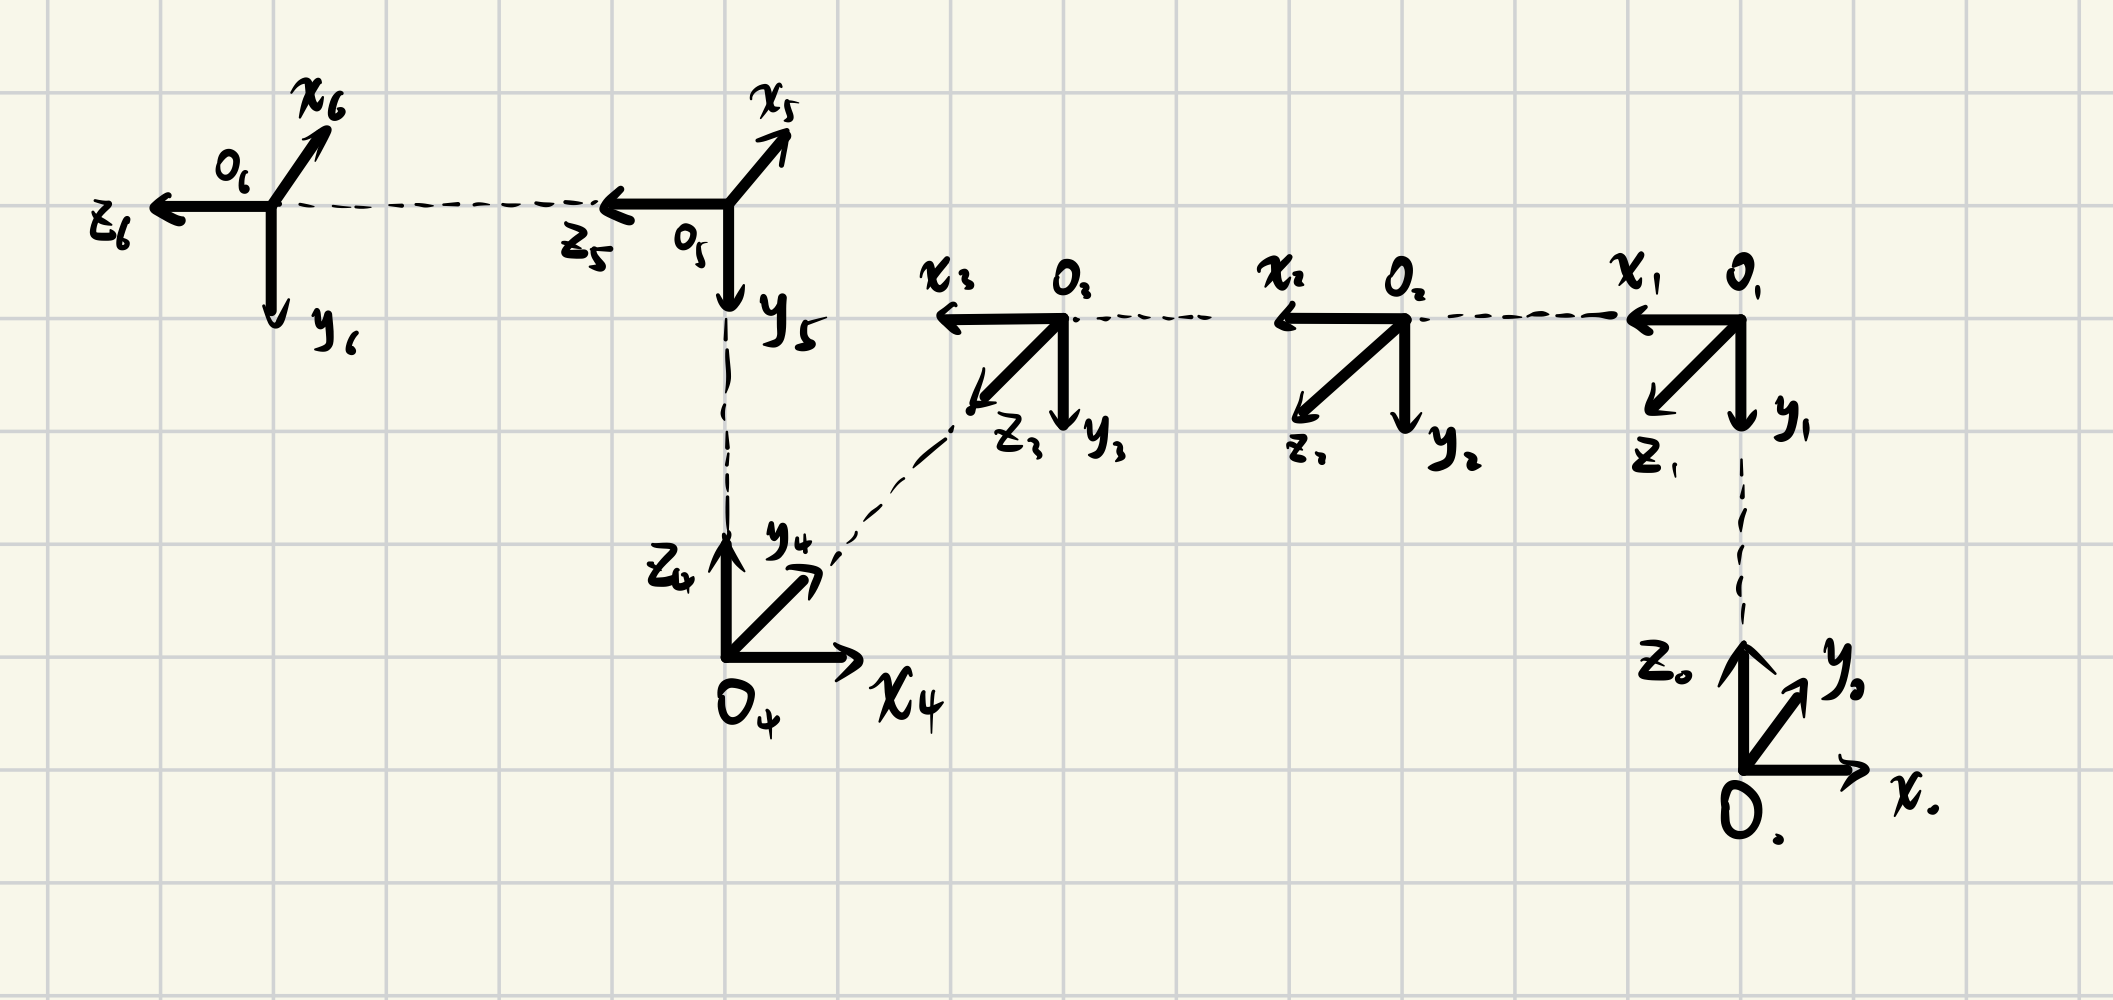
\includegraphics[width=1.0\textwidth]{asset/DH_coor.png}
    \caption{DH坐标系}
\end{figure}
\begin{table}[h]
    \centering
    \begin{tabular}{|c|c|c|c|c|}
        \hline
        连杆i & \(\theta_i\) & \(d_i\) & \(a_i\) & \(\alpha_i\) \\
        \hline
        1 & $180^\circ$ & 162.5 & 0 & $-90^\circ$ \\
        \hline
        2 & 0 & 0 & 425 & 0 \\
        \hline
        3 & 0 & 0 & 392.2 & 0 \\
        \hline
        4 & $180^\circ$ & 133.3 & 0 & $-90^\circ$ \\
        \hline
        5 & $90^\circ$ & 99.7 & 0 & $-90^\circ$ \\
        \hline
        6 & 0 & 99.6 & 0 & 0 \\
        \hline
    \end{tabular}
    \caption{DH参数表}
\end{table}
\vspace{1em}

(2)
\[
\begin{aligned}
{}^0T_1 &= \begin{bmatrix}
        \cos(\theta_1 + 180^\circ) & -\sin(\theta_1 + 180^\circ) & 0 & 0 \\
        \sin(\theta_1 + 180^\circ) & \cos(\theta_1 + 180^\circ) & 0 & 0 \\
        0 & 0 & 1 & 0 \\
        0 & 0 & 0 & 1 \\
        \end{bmatrix}
        \begin{bmatrix}
        1 & 0 & 0 & 0 \\
        0 & 1 & 0 & 0 \\
        0 & 0 & 1 & 162.5 \\
        0 & 0 & 0 & 1 \\
        \end{bmatrix}
        \begin{bmatrix}
        1 & 0 & 0 & 0 \\
        0 & \cos(-90^\circ) & -\sin(-90^\circ) & 0 \\
        0 & \sin(-90^\circ) & \cos(-90^\circ) & 0 \\
        0 & 0 & 0 & 1 \\
        \end{bmatrix} \\
        &= \begin{bmatrix}
        -\cos\theta_1 & 0 & \sin\theta_1 & 0 \\
        -\sin\theta_1 & 0 & -\cos\theta_1 & 0 \\
        0 & -1 & 0 & 162.5 \\
        0 & 0 & 0 & 1 \\
        \end{bmatrix} \\[1em]
{}^1T_2 &= \begin{bmatrix}
        \cos\theta_2 & -\sin\theta_2 & 0 & 0 \\
        \sin\theta_2 & \cos\theta_2 & 0 & 0 \\
        0 & 0 & 1 & 0 \\
        0 & 0 & 0 & 1 \\
        \end{bmatrix}
        \begin{bmatrix}
        1 & 0 & 0 & 425 \\
        0 & 1 & 0 & 0 \\
        0 & 0 & 1 & 0 \\
        0 & 0 & 0 & 1 \\
        \end{bmatrix} \\
        &= \begin{bmatrix}
        \cos\theta_2 & -\sin\theta_2 & 0 & 425\cos\theta_2 \\
        \sin\theta_2 & \cos\theta_2 & 0 & 425\sin\theta_2 \\
        0 & 0 & 1 & 0 \\
        0 & 0 & 0 & 1 \\
        \end{bmatrix} \\[1em]
{}^2T_3 &= \begin{bmatrix}
        \cos\theta_3 & -\sin\theta_3 & 0 & 0 \\
        \sin\theta_3 & \cos\theta_3 & 0 & 0 \\
        0 & 0 & 1 & 0 \\
        0 & 0 & 0 & 1 \\
        \end{bmatrix}
        \begin{bmatrix}
        1 & 0 & 0 & 392.2 \\
        0 & 1 & 0 & 0 \\
        0 & 0 & 1 & 0 \\
        0 & 0 & 0 & 1 \\
        \end{bmatrix} \\
        &= \begin{bmatrix}
        \cos\theta_3 & -\sin\theta_3 & 0 & 392.2\cos\theta_3 \\
        \sin\theta_3 & \cos\theta_3 & 0 & 392.2\sin\theta_3 \\
        0 & 0 & 1 & 0 \\
        0 & 0 & 0 & 1 \\
        \end{bmatrix} \\
\end{aligned}
\]

\[
\begin{aligned}
{}^3T_4 &= \begin{bmatrix}
        \cos(\theta_4 + 180^\circ) & -\sin(\theta_4 + 180^\circ) & 0 & 0 \\
        \sin(\theta_4 + 180^\circ) & \cos(\theta_4 + 180^\circ) & 0 & 0 \\
        0 & 0 & 1 & 0 \\
        0 & 0 & 0 & 1 \\
        \end{bmatrix}
        \begin{bmatrix}
        1 & 0 & 0 & 0 \\
        0 & 1 & 0 & 0 \\
        0 & 0 & 1 & 133.3 \\
        0 & 0 & 0 & 1 \\
        \end{bmatrix}
        \begin{bmatrix}
        1 & 0 & 0 & 0 \\
        0 & \cos(-90^\circ) & -\sin(-90^\circ) & 0 \\
        0 & \sin(-90^\circ) & \cos(-90^\circ) & 0 \\
        0 & 0 & 0 & 1 \\
        \end{bmatrix} \\
        &= \begin{bmatrix}
        -\cos\theta_4 & 0 & \sin\theta_4 & 0 \\
        -\sin\theta_4 & 0 & -\cos\theta_4 & 0 \\
        0 & -1 & 0 & 133.3 \\
        0 & 0 & 0 & 1 \\
        \end{bmatrix} \\
{}^4T_5 &= \begin{bmatrix}
        \cos(\theta_5 + 90^\circ) & -\sin(\theta_5 + 90^\circ) & 0 & 0 \\
        \sin(\theta_5 + 90^\circ) & \cos(\theta_5 + 90^\circ) & 0 & 0 \\
        0 & 0 & 1 & 0 \\
        0 & 0 & 0 & 1 \\
        \end{bmatrix}
        \begin{bmatrix}
        1 & 0 & 0 & 0 \\
        0 & 1 & 0 & 0 \\
        0 & 0 & 1 & 99.7 \\
        0 & 0 & 0 & 1 \\
        \end{bmatrix}
        \begin{bmatrix}
        1 & 0 & 0 & 0 \\
        0 & \cos(-90^\circ) & -\sin(-90^\circ) & 0 \\
        0 & \sin(-90^\circ) & \cos(-90^\circ) & 0 \\
        0 & 0 & 0 & 1 \\
        \end{bmatrix} \\
        &= \begin{bmatrix}
        -\sin\theta_5 & 0 & -\cos\theta_5 & 0 \\
        \cos\theta_5 & 0 & -\sin\theta_5 & 0 \\
        0 & -1 & 0 & 99.7 \\
        0 & 0 & 0 & 1 \\
        \end{bmatrix} \\
{}^5T_6 &= \begin{bmatrix}
        \cos\theta_6 & -\sin\theta_6 & 0 & 0 \\
        \sin\theta_6 & \cos\theta_6 & 0 & 0 \\
        0 & 0 & 1 & 0 \\
        0 & 0 & 0 & 1 \\
        \end{bmatrix}
        \begin{bmatrix}
        1 & 0 & 0 & 0 \\
        0 & 1 & 0 & 0 \\
        0 & 0 & 1 & 99.6 \\
        0 & 0 & 0 & 1 \\
        \end{bmatrix} \\
        &= \begin{bmatrix}
        \cos\theta_6 & -\sin\theta_6 & 0 & 0 \\
        \sin\theta_6 & \cos\theta_6 & 0 & 0 \\
        0 & 0 & 1 & 99.6 \\
        0 & 0 & 0 & 1 \\
        \end{bmatrix}
\end{aligned}
\]

故
\[
\begin{aligned}
{}^0T_1 &= \begin{bmatrix}
            -\cos\theta_1 & 0 & \sin\theta_1 & 0 \\
            -\sin\theta_1 & 0 & -\cos\theta_1 & 0 \\
            0 & -1 & 0 & 162.5 \\
            0 & 0 & 0 & 1 \\
            \end{bmatrix} \\
{}^1T_4 &= {}^1T_2 \cdot {}^2T_3 \cdot {}^3T_4 = \begin{bmatrix}
            -\cos(\theta_2 + \theta_3 + \theta_4) & 0 & \sin(\theta_2 + \theta_3 + \theta_4) & 425\cos\theta_2 + 392.2\cos(\theta_2 + \theta_3) \\
            -\sin(\theta_2 + \theta_3 + \theta_4) & 0 & -\cos(\theta_2 + \theta_3 + \theta_4) & 425\sin\theta_2 + 392.2\sin(\theta_2 + \theta_3) \\
            0 & -1 & 0 & 133.3 \\
            0 & 0 & 0 & 1 \\
            \end{bmatrix} \\
{}^4T_6 &= {}^4T_5 \cdot {}^5T_6 = \begin{bmatrix}
            -\sin\theta_5\cos\theta_6 & \sin\theta_5\sin\theta_6 & -\cos\theta_5 & -99.6\cos\theta_5 \\
            \cos\theta_5\cos\theta_6 & -\cos\theta_5\sin\theta_6 & -\sin\theta_5 & -99.6\sin\theta_5 \\
            -\sin\theta_6 & -\cos\theta_6 & 0 & 99.7 \\
            0 & 0 & 0 & 1 \\
            \end{bmatrix} \\
\end{aligned}
\]
\vspace{1em}

(3)
将\([\theta_1 \; \theta_2 \; \theta_3 \; \theta_4 \; \theta_5 \; \theta_6] = [16^\circ \; -124^\circ \; 63^\circ \; 152^\circ \; 88^\circ \; -166^\circ]\)代入得
\[
\begin{aligned}
{}^0T_6 &= {}^0T_1 \cdot {}^1T_4 \cdot {}^4T_6 \\
        &= \begin{bmatrix}
            -0.9612 & 0 & 0.2756 & 0 \\
            -0.2756 & 0 & -0.9612 & 0 \\
            0 & -1 & 0 & 162.5 \\
            0 & 0 & 0 & 1
            \end{bmatrix}
            \begin{bmatrix}
            0.0174 & 0 & 0.9998 & -47.5146 \\
            -0.9998 & 0 & 0.0174 & -695.3668 \\
            0 & -1 & 0 & 133.3 \\
            0 & 0 & 0 & 1
            \end{bmatrix} \\
            &\begin{bmatrix}
            0.9697 & -0.2417 & -0.0348 & -3.4759 \\
            -0.0338 & 0.0084 & -0.9993 & -99.5393 \\
            0.2419 & 0.9703 & 0 & 99.7 \\
            0 & 0 & 0 & 1
            \end{bmatrix} \\
        &= \begin{bmatrix}
            -0.2397 & -0.9308 & 0.2760 & 14.0886 \\
            -0.1038 & -0.2581 & -0.9605 & -238.1828 \\
            0.9653 & -0.2587 & -0.0349 & 852.6513 \\
            0 & 0 & 0 & 1
            \end{bmatrix}
\end{aligned}
\]
\vspace{0.5em}

位置矢量
\[
P = \begin{bmatrix}
    14.0886 \\ -238.1828 \\ 852.6513 
    \end{bmatrix}
\]

对于XYZ欧拉角有
\[
\begin{aligned}
    R &= \begin{bmatrix}
        1 & 0 & 0 \\
        0 & \cos\alpha & -\sin\alpha \\
        0 & \sin\alpha & \cos\alpha \\
        \end{bmatrix}
        \begin{bmatrix}
        \cos\beta & 0 & \sin\beta \\
        0 & 1 & 0 \\
        -\sin\beta & 0 & \cos\beta \\
        \end{bmatrix}
        \begin{bmatrix}
        \cos\gamma & -\sin\gamma & 0 \\
        \sin\gamma & \cos\gamma & 0 \\
        0 & 0 & 1 \\
        \end{bmatrix} \\
        &= \begin{bmatrix}
        -0.2397 & -0.9308 & 0.2760 \\
        -0.1038 & -0.2581 & -0.9605 \\
        0.9653 & -0.2587 & -0.0349 \\
        \end{bmatrix}
\end{aligned}
\]

解得
\[
\beta = \arcsin(0.2760) = 16.02^\circ \text{ 或 } \beta = 180^\circ - 16.02^\circ = 163.98^\circ
\]

当 $\beta_1 = 16.02^\circ$ 时
\[
\begin{aligned}
    \alpha_1 &= \arctan2\left(-\frac{a_{23}}{\cos\beta_1}, \frac{a_{33}}{\cos\beta_1}\right) = 92.08^\circ \\
    \gamma_1 &= \arctan2\left(-\frac{a_{12}}{\cos\beta_1}, \frac{a_{11}}{\cos\beta_1}\right) = 104.45^\circ
\end{aligned}
\]

当 $\beta_2 = 163.98^\circ$ 时
\[
\begin{aligned}
    \alpha_2 &= \arctan2\left(-\frac{a_{23}}{\cos\beta_2}, \frac{a_{33}}{\cos\beta_2}\right) = -87.92^\circ \\
    \gamma_2 &= \arctan2\left(-\frac{a_{12}}{\cos\beta_2}, \frac{a_{11}}{\cos\beta_2}\right) = -75.55^\circ
\end{aligned}
\]

综上,XYZ欧拉角解为
\[
\Psi = \begin{bmatrix}
        92.08^\circ \\ 16.02^\circ \\ 104.45^\circ
        \end{bmatrix} 
        \text{ 或 } 
\Psi = \begin{bmatrix}
        -87.92^\circ \\ 163.98^\circ \\ -75.55^\circ
        \end{bmatrix}
\]
\end{document} 
